
\documentclass[journal]{IEEEtran}

\usepackage{epsfig,graphicx,lineno,amssymb,mdwmath,array,amsmath}
\usepackage{subfigure}
\usepackage{multirow}
\usepackage{xcolor}
\usepackage{cite}
\usepackage{epstopdf}
\usepackage{latexsym, bm}
\usepackage{algorithm}
\usepackage{algorithmicx}
\usepackage{algpseudocode}
\usepackage[utf8]{inputenc}
\usepackage[T1]{fontenc}
\usepackage{listings}

\definecolor{pblue}{rgb}{0.13,0.13,1}
\definecolor{pgreen}{rgb}{0,0.5,0}
\definecolor{pred}{rgb}{0.9,0,0}
\definecolor{pgrey}{rgb}{0.46,0.45,0.48}
\lstset{
  language=Java,
  frame=single,
  emph={enableRssiPolling},
%   emphstyle=\textbf,
  emphstyle=\color{red},
  showspaces=false,
  showtabs=false,
  breaklines=true,
  showstringspaces=false,
  breakatwhitespace=true,
  commentstyle=\color{pgreen},
  keywordstyle=\color{pblue},
  stringstyle=\color{pred},
%   basicstyle=\ttfamily,
  basicstyle=\small,
  stringstyle=\ttfamily,
  moredelim=[il][\textcolor{pgrey}]{$1$},
  moredelim=[is][\textcolor{pgrey}]{\%\%}{\%\%},
  numbers=left, numberstyle=\tiny, stepnumber=1, numbersep=5pt
}


\newtheorem{mydef}{Definition}
\newtheorem{mylem}{Lemma}
\newtheorem{mythm}{Theorem}
\newtheorem{cor}{Corollary}

\hyphenation{op-tical net-works semi-conduc-tor}

\makeatletter       %for algorithm
\def\BState{\State\hskip-\ALG@thistlm} %for algorithm
\makeatother %for algorithm

\algnewcommand\algorithmicswitch{\textbf{switch}}
\algnewcommand\algorithmiccase{\textbf{case}}

\algblockdefx[Name1]{SWITCH}{ENDSWITCH}%
%   [1]{\textbf{switch} #1 \textbf{do}}%
 [1]{\textbf{switch} #1}%
  {\textbf{end switch}}
\algblockdefx[Name2]{CASE}{ENDCASE}%
  [1]{\textbf{case} #1 \textbf{do}}%
  {\textbf{end case}}

\begin{document}
%
% paper title
% can use linebreaks \\ within to get better formatting as desired
% Do not put math or special symbols in the title.
\title{An Rssi-Based Wi-Fi Download Management Approach for Energy Saving on Smartphones}
%
\author{Lunde~Chen,
        ~Huan~Li*,~\IEEEmembership{Member,~IEEE,}% <-this % stops a space
\thanks{*Corresponding Author: H. Li,  is with the School
of Computer Science and Engineering, Beihang University, Beijing,
China 100191,  e-mail: lihuan@buaa.edu.cn.}% <-this % stops a space
\thanks{L. Chen is with with the School of Computer Science and Engineering and Ecole Centrale de P\'{e}kin, Beihang University, Beijing, China 100191.}% <-this % stops a space
\thanks{Manuscript received September 15, 2014.}}

% The paper headers
\markboth{IEEE EMBEDDED SYSTEMS LETTERS}%%Journal of \LaTeX\ Class Files,~Vol.~11, No.~4, December~2012}%
{Shell \MakeLowercase{\textit{et al.}}: Bare Demo of IEEEtran.cls for Journals}

\maketitle

\begin{abstract}
Smartphones are emerging as a particularly appealing platform for network applications, 
espacially through the Wi-Fi interface. However,
Wi-Fi entails considerable energy consumption and smartphones
are bottlenecked by their battery capacity. Finding ways to reduce 
energy consumption of Wi-Fi is more than critical.
In this paper, we address the problem of energy saving of Wi-Fi 
with regarding to Rssi. Through extensive experiments, we investigate how 
Rssi influences energy consumption. Based on our experimental findings, 
we propos a novel Rssi-based Wi-Fi download management approach for energy saving on smartphones
which is simple but highly elaborate.
Simulations prove that our approach is effective and can achieve more than 100\% energy saving, 
both in a constantly moving scenario and in a stationary-moving scenario.
\end{abstract}

% Note that keywords are not normally used for peerreview papers.
\begin{IEEEkeywords}
Rssi, Energy saving, algorithm.
\end{IEEEkeywords}

\IEEEpeerreviewmaketitle

\section{Introduction}

% \IEEEPARstart{G}{uidance}: This paragraph is to address 1) the growth of the multimedia applications on smartphone 
% [Need some data evidence],
% and most need download large files, e.g., app tar files and movies etc.
% 2) the wifi access requirements for those applications, and 
% 3) major Wifi properties and the impact on the critical energy issues on resource-constrained smartphones. 
% {[\bf Guidance:]}  
% 1) The most widely used energy-efficient wifi access strategies, such as prediction sleeping methods are introduced here, 
% 2) The limits or problems of those strategies.
 \IEEEPARstart{S}{martphones} are becoming increasingly popular because of
their capabilities and functionalities and have emerged as a particularly appealing platform for network applications, 
espacially through the Wi-Fi interface.
However, these light-weighted and easy-to-carry devices are constrained by their limited battery capacity.
Considering that people use their smartphones to download large files such as movies, documents and apk tar files, 
in a stationary scenario or in a moving scenario,
we address in this paper the energy consumption of downloading files via Wi-Fi and how to achieve better energy efficiency, 
with regarding to Rssi.
\\
\indent
We first investigate the relationship between the energy consumption and Rssi and conclude that Rssi has a major 
impact on the energy consumption, and a Rssi-based Wi-Fi download management scheme is needed to achieve good energy efficiency. 
However, one of the key challenges is that constantly varying nature of Rssi. For example, as presented in [1],
at a distance of 24 m, Rssi values between -40 and -84 dBm are encountered. Our experiments show that the weaker Rssi is, 
the greater its variation will be. This observation in line with the work done in [2]. Accurate Rssi measurement [3] may be helpful,  
but this involves detecting trends in Rssi values, detecting changes in transmission power, or detecting motions, which causes extra energy overhead. 
As the relationship between Rssi and energy consumption is threshold-based, 
we are able to conceive a simpler solution.
\\
\indent
Prediction-based algorithm such as [4] may achieve good performance in a constantly moving scenario. In our algorithm, 
we take the opposite way, i.e. the making-sure strategy.
Instead of predicting Rssi of the next moment, we make sure that the smartphone is truly in a strong signal 
area when starting downloading files, and make sure that the signal is truly degraded when stopping downloading files.
In this way, we not only leverage the varying nature of Rssi, making each decision of starting or stopping downloads wiser and more reasonnable, 
but also avoid constantly stopping and restarting downloads, causing 
significant energy overhead of interrupting and reestablishing TCP connections as well as tail energy.
\\
\indent
We also take into the geometric characteristics of Wi-Fi signal and moving smartphones when conceiving our algorithm. We conduct Monte-Carlo
simulations and show the effectiveness of our algorithm.
% {[\bf Guidance:]} The contributions of this paper:
% 1) extensive experiments to evaluate the relationship of rssi and the energy consumption, 
% 2) propose a novel Rssi-based wifi access management algorithm, 
% 3) effectiveness evaluation using simulations.
\\
\indent
The main contributions of this paper are as follows:
\\
\indent
(1) We conduct extensive experiments to evaluate the relationship of rssi and the energy consumption.
\\
\indent
(2) We propose a novel Rssi-based wifi access management algorithm, leveraging 
the inaccuracy of one measurement of Rssi and the additional energy consumption of pausing and restarting a download, taking
into the geometric characteristics of Wi-Fi signal.
\\
\indent
(3) We conduct effectiveness evaluation using simulations and show the effectiveness of our algorithm.
\\
\indent
The rest of this article is organized as follows. We review some substantial works that
focus on energy saving of Wi-Fi in Section II. In Section III,
we describe our experimental settings for measuring the energy consumption of downloading a file at different Rssi and present our results.
Our algorithm for energy saving is described in Section IV, and simulation results of our algorithm are given in Section V.
We conclude our work in Section VI.

\section{Related Works}
Energy optimization for smartphones has attracted considerable attention in recent years, and lots of researches 
have been done on the energy consumption of Wi-Fi. 
\\
\indent
Tan et al. [5] proposed power save mode
(PSM) throttling, an application-independent protocol, which reshapes TCP traffic into periodic bursts
with the same average throughput as the server transmission rate. Clients accurately
predict the arriving time of packets, and turn on/off the wireless interfaces accordingly.
PSM-throttling can minimize power consumption on TCP-based bulk traffic by effectively
utilizing available Internet bandwidth without degrading the performance of application
perceived by the user.
\\
\indent
Fahad R. Dogar et al. [6] proposed Catnap, a system that exploits high bandwidth wireless interfaces
by combining small gaps between packets into meaningful sleep intervals, thereby allowing the
NIC as well as the device to doze off. Catnap targets data
oriented applications, such as web and file transfers, which
can afford delay of individual packets as long as the overall
transfer times do not increase. Catnap is implemented as an application independent 
proxy to decouple wired and wireless segments, and schedules ADU 
transmissions on the wireless side using hints regarding the 
application workload.
% \\
% \indent
% In [4] SiFi (silence prediction based WiFi energy adaptation), 
% which exploits VoIP silence for WiFi energy savings in smart phones. 
% SiFi examines audio streams from phone calls and
% tracks when silence periods start and stop. This data is stored
% in a prediction model. Using this historical data, they predict
% the length of future silence periods and place the WiFi radio
% to sleep during these periods. 
% \\
% \indent
% In [5] Anatomy of WiFi Access Traffic of Smartphones and Implications for Energy Saving Techniques
\\
\indent
In [7], Young-Seol Lee and Sung-Bae Cho proposed a context-aware battery management
system that uses probabilistic models to infer a 
user’s situation with low power sensors such as acceleration and
orientation and controls components that consume a large amount
of energy such as screen and Wi-Fi interface. 
For example, when the system infers that 
the user goes out, it turns off Wi-Fi automatically. 
However, the authors didn't take into consideration 
the energy overhead of closing and reopening the Wi-Fi interface, which is 
more than 30 minutes of the energy consumption of keeping it open.
\\
\indent
In [8], Jian Li et al. investigate the key
factors influencing Wi-Fi energy consumption, and propose three
energy management schemes: 1) dynamic control of Wi-Fi on/off
interface; 2) improve communication efficiency via application
packing; and 3) elongation of Wi-Fi Power Save Mode (PSM)
via application alignment under mixed application workload.
They design and test their solution as a device-side application
utilizing general system process scheduling and network firewall
techniques. However, their work regarding to Rssi didn't take 
into consideration the energy consumption characteristics, 
geometric characteristics and variation characteristics of Wi-Fi.
\\
\indent
Previous work that is the most similar to ours is [4], which proposed a non-parametric Rssi prediction 
based energy-saving scheme for moving smartphones. 
By periodically monitoring Rssi in diverse network environments, 
their proposed scheme applies weighted scatter plot smoothing and kernel
moving average algorithms to adaptively adjust file downloading and video streaming rates.
However, the KMA prediction model  
that they adopted consumes much energy, causing a significant energy overhead. Besides, 
in the interval of [-90dBm, -70dBm], the variation of Rssi is more than 6dBm, and the accuracy of prediction models such as KMA 
can be greatly degraded. As they showed, in a fixed location scenario, 
their scheme may consume almost 100\% more energy than if no prediction or adaption adopted for downloading files.
\section{Evaluation of Rssi and Energy Consumption}
%\subsection{Settings and Methodology}
%{[\bf Guidance:]} Experimental environment and settings
%\subsection{Experimental Setup for Rssi Charactirization}

\subsection{Experimental Setup for Power Measurement}
This section describes the experimental setup for power measurement. 
\\
\indent
{\bf Experimental Setup and Measurement Technology}: The DUT (Device Under Test) 
is a Huawei 8950D running Android 4.0 with superuser access, supporting IEEE 802.11 n/b/g. It's 
equiped with a double-core 1.2GHz Snapdragon MSM8225 CPU and 768MB RAM. We use a Monsoon Power Monitor [9] for power measurement.
The Monsoon Power Monitor supplies a stable voltage of 3.7V to the DUT and samples the power consumption at a rate of 5KHz. 

{\bf Measurement Methodology}: To perform the download, an application (WiDownload) that downloads files 
using the DownloadManager API provided by Android is developped and installed in the DUT. 
We also cross compile Iptables and Tcpdump and install them into the DUT as local libararies.
% Iptables is used to block the Internet access of unrelated applications to avoid interference traffic. 
% Tcpdump is used to analyze traffic performance such as RTT, packet loss and throughput. 
\\  
\indent
We adjust the distance between the DUT and the AP to get different Rssi. 
When we perform measurements, we keep all instruments at fixed location. 
We use Iptables to block the Internet access of all applications 
except that of WiDownload so that no interference traffic is introduced. 
During the download, the screen is off and the WifiLock is aquired. 
\\  
\indent We measure the power consumed for 
completing downloading a file of 11.4 Mb. After this, we perform the same download at the same fixed location, but with 
Tcpdump running to dump traffic information. Each measurement is repeated 3 times. After that, we move the instruments to 
another location where Rssi is different and reconduct the experiment. 

%{[\bf Guidance:]} We measure....

\subsection{Measurement Results}
%Put the figures and analysis here.
%\\
%\indent 
Figure 1 shows the power consumption for download a file at strong (-30 dBm) and weak (-84 dBm) Rssi.
Figure 2 and 3 are the corresponding traffic throughputs. Comparing the two, we can infer that the energy consumption 
for downloading files can be assumed to be proportional to the time it takes to finish the download. 
Rssi influences the the energy consumption for downloading files mainly due to its impact on the throughput.
The whole dataset of the relationship between Rssi (averaged over time) and the energy consumption is plotted in Figure 4.


% if error, type << pdflatex --shell-escape Version-1.tex >> in Terminal
\begin{figure}
\centering
% \captionsetup{justification=centering}
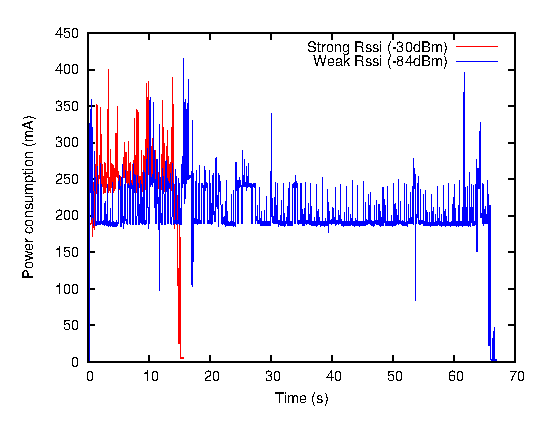
\includegraphics[scale=1]{energy_comparision.eps}
\caption{Power consumption for downloading a file of 11.4Mb in different Rssi}
\end{figure}

\begin{figure}
\centering
% \captionsetup{justification=centering}
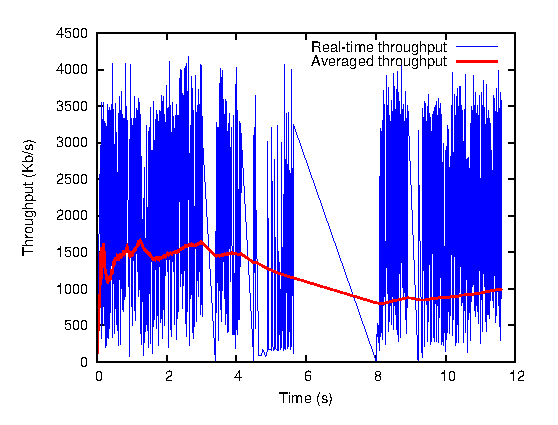
\includegraphics[scale=0.95]{strong_traffic.eps}
\caption{Throughput in strong Rssi (-30dBm)}
\end{figure}

\begin{figure}
\centering
% \captionsetup{justification=centering}
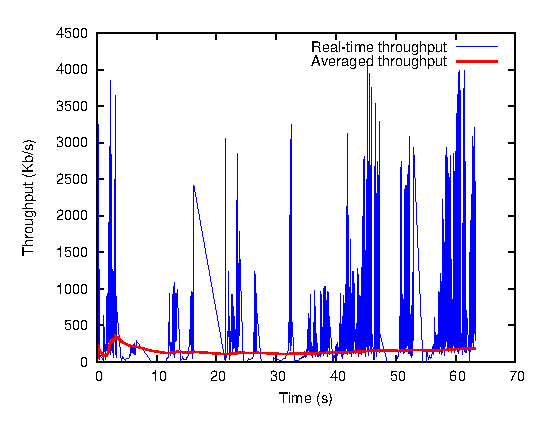
\includegraphics[scale=0.95]{weak_traffic.eps}
\caption{Throughput in weak Rssi (-84dBm)}
\end{figure}

\begin{figure}
\centering
% \captionsetup{justification=centering}
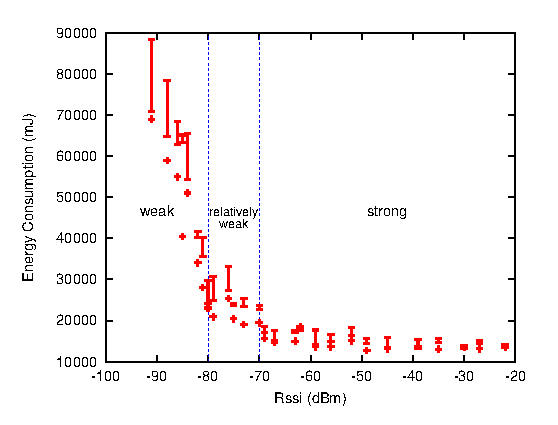
\includegraphics[scale=0.95]{rssi_energy.eps}
\caption{Energy Consumption in different Rssi}
\end{figure}

\indent 
We conclude that when Rssi is higher than -70dBm, 
the energy consumption for the download is limited and independent of Rssi.
When Rssi is between -70dBm and -80dBm, the energy consumption for the download increases as Rssi becomes weaker, but not so significantly.  
When Rssi is below -80dBm, the energy consumption for downloading files increases dramatically. 
\\
\indent 
Comparing the duration of throughput and energy consumption, we can see that the energy consumption duration is always 3-5 seconds longer than that of 
throughput. To further investigate this phenomenon, we use WiDownload to download a 22KB file, which is downloaded in less in 1 second, but the duration of 
energy consumption is more than 6 seconds. We conclude that Wi-Fi, as with 3G, introduces
significant tail energy [10]. We can see that tail energy represents a great overhead if the download session is short.
\section{Rssi-based Wi-Fi Download Management Algorithm}
\subsection{Requirements for a good Rssi-based Download Management Algorithm}
As Rssi has an significant impact on the energy consumption of the Wi-Fi downloading, one may consider closing the Wi-Fi interface 
when the Wi-Fi signal is weak and reopening it when the Wi-Fi signal is strong. However, our experiments show that 
closing and openning the Wi-Fi interface consumes much energy,  3700 mJ and 4300 mJ respectively, shown in Figure 5. 
Keeping the Wi-Fi interface open, on the other hand, consumes only 3.95 mW overhead. 
The energy consumption of closing and openning the Wi-Fi interface is equal to that of keeping the Wi-Fi open for 2025 seconds.
Besides, keeping the Wi-Fi open allows to monitor Wi-Fi condition and adjust the smartphone's networking behaviors accordingly.
In designing our Rssi-based download management algorithm, we keep the Wi-Fi interface open.
\\
\indent
A good Rssi-based download management algorithm should take into consideration the 2 following major characteristics of Rssi of Wi-Fi. 
\\
\indent
First, we should also take into consideration the geometric characteristics of the Wi-Fi signal. Our measurements show that the distance 
of Rssi range of -70dBm to -80dBm is 4-10 meters, depending on the obstacles present in the Wi-Fi environment. 
As a person walks typically around 1.5m/s, not necessarily against the rayon direction 
of the Wi-Fi signal of AP, the phone has always sufficient time to adjust its download behavior to the Wi-Fi signal change within one sampling period, 
2 seconds in our algorithm.
\\
\indent
Second, when the Wi-Fi signal is weak or relatively weak, the variation of Rssi measured is significant. Each measurement of Rssi can thus be inaccurate.
Adapting the download behavior to Rssi change should leave space for the verification of Rssi.
\\
\indent
A good Rssi-based download management algorithm should also take into consideration the 2 following major characteristics of energy consumption of smartphones at different Rssi of Wi-Fi:
\\
\indent
First, when Rssi is higher than -70dBm, the 
energy consumption for downloading files varies little and can be considered as constant. 
When Rssi is between -70dBm and -80dBm, the energy consumption for downloading files 
increases but not so significantly. So we can tolerate some time of download spent in the range of -70dBm and -80dBm if this could lead 
to better overall energy-saving strategy.
\\
\indent
Second, we should avoid frequent transition between download and not download. In the one hand, interrupting and 
reestablishing a TCP connection can waste much energy and influence the download
efficiency. In the other hand, each time a download is stopped, the Wi-Fi interface will continue to consume tail energy for 3-5 seconds, as we have presented in Sction II. 
%\\
%\indent 
%(Tail Energy...)

\begin{figure}
\centering
% \captionsetup{justification=centering}
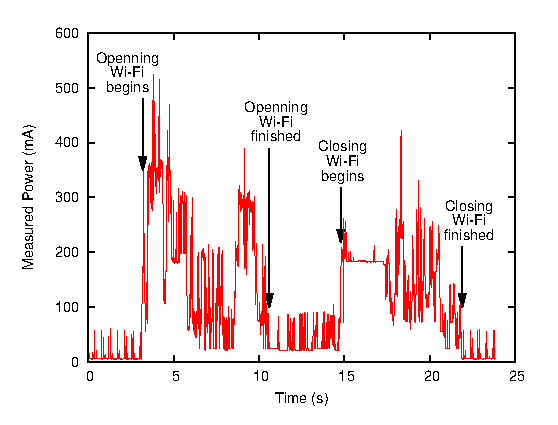
\includegraphics[scale=0.95]{energy_open_close_wifi.eps}
\caption{Energy Consumption of openning and closing Wi-Fi interface}
\end{figure}
\begin{figure}
\centering
% \captionsetup{justification=centering}
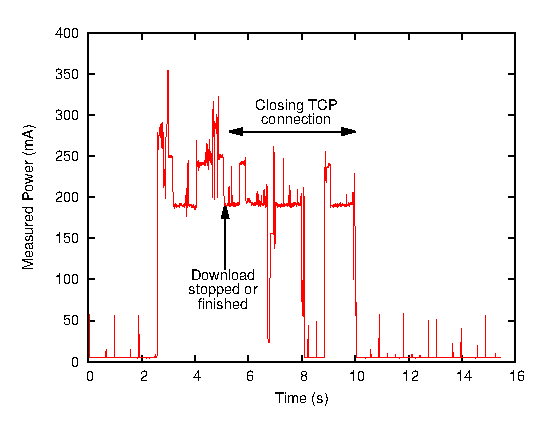
\includegraphics[scale=0.95]{energy_Download_22KB.eps}
\caption{Energy Consumption of downloading a 22KB file}
\end{figure}
\subsection{Our Decision-Tree-Based Algorithm}
Based on our finding in experiments, we are able to conceive the Rssi-based Wi-Fi Download Management Algorithm. 
We divide Wi-Fi signal strength measured by the smartphone into 3 categories: strong, relatively weak and weak, 
according to its impact on energy consumption:
\\
\indent 
(A) Strong:           Rssi $>=$ -70dBm
\\
\indent 
(B) Relatively weak:  Rssi $\in$ [-80dBm, -70dBm)
\\
\indent 
(C) Weak: 	      Rssi $<$ -80dBm
\\
\indent 
We define 3 different perceptions of Wi-Fi: \textit{good}, \textit{acceptable}, \textit{bad}. However,
what's subtle is that the perception of Wi-Fi is not a simple mapping
of the signal strength of Wi-Fi, but obtained dynamically according to previous perception and the Rssi measured, as shown in Figure 5.
\\
\indent
According to the current perception of Wi-Fi, we adjust the download strategy adaptively. The basic idea 
is to start downloading files when the perception of Wi-Fi is \textit{good}, and to stop the download when the perception is \textit{bad}. If the perception 
is \textit{acceptable}, we continue the download if the download is running, and stay in the paused stated if the download is paused.
\\
\indent 
Our Rssi-based Wi-Fi download management algorithm works iteratively in three steps: update current perception of Wi-Fi, 
ajust download according to the current perception of Wi-Fi and sleep for 1 second. The pseudo-code in given in Algorithm 1.
\begin{algorithm}
\caption{Rssi-based Download Management Algorithm}\label{all}
\begin{algorithmic}[1]
% \Procedure{RssiBasedDownloadControl}{}
\While {true}
\State /**Update current perception of Wi-Fi,  
\State  *as shown in Figure 7 */
\State update\_perception()
\If {curr\_perception is \textit{good}}
\State start\_download()
\ElsIf {curr\_perception is \textit{bad}}
\State stop\_download()
\EndIf
\State prev\_perception $\gets$ curr\_perception
\State sleep() //sleep for 1 second
\EndWhile
% \EndProcedure
\end{algorithmic}
\end{algorithm}
We incorporate these ideas in our algorithm mainly in the decision tree for updating current perception of Wi-Fi. 
The path 1, 3, 6 and 9 is easy to understand. Here are further analysis of the 
five other paths:
\\
\indent
(a) Path 2: 
The previous perception is \textit{good}, according to Algorithm 2, the phone is downloading files. 
As each Rssi measurement could be inaccurate, the Rssi measured is not sure indicator that the Wi-Fi signal is degraded. 
We set Path 2 to be \textit{acceptable}, so that the decision-making is to be performed at the next iteration (to make sure). If the 
relatively weak Rssi is due to measurement variation, 
the next moment Path 4 will be taken and the perception will be updated to be \textit{good}.
In this way, the download is not interrupted and the energy overhead of reestablishing TCP connection is spared. If the relatively
weak Rssi is due to the user moving to where the signal is degraded, the path 5 or 6 will be taken the next moment and the download will 
be stopped. 
\\
\indent
(b) Path 4:
As the previous perception  is \textit{acceptable}, the perception prior to the previous moment could be \textit{good} or \textit{bad}. 
If the perception prior to the previous moment is \textit{good}, the Path 2 is taken at the previous moment. 
So the sequence of the 3 most recent Rssi measured is: strong $\to$  relatively strong 
$\to$ strong. The download is not interrupted. If the perception prior to the previous moment is \textit{bad}, then the sequence of the 3 most recent Rssi measured 
is: relatively weak or weak $\to$  strong $\to$  strong. It's a good indicator the phone comes into the strong Wi-Fi zone from
a relatively distant location where the Wi-Fi is weak or relatively weak. And the \textit{good} set here will trigger the download to start.
\\
\indent
(c) Path 5:
As the previous perception is \textit{acceptable}, 
the perception prior to the previous moment could be \textit{good} or \textit{bad}.
If the perception prior to the previous moment is \textit{good}, the sequence of the 3 most recent Rssi measured is: strong $\to$  relatively weak $\to$  relatively Weak, 
which is a good indicator that we get far away from the AP. As Path 5 is set to be \textit{bad}, the download will be stopped and waste of energy in a 
degraded Wi-Fi is avoided. If the perception prior to the previous moment is \textit{bad}, then the download is not started and the paused state of download will be continued.
\\
\indent
(d) Path 7:
The jump of the Rssi measured from weak to strong is rare, so this could be caused by the accidental measurement error. Not sure about the real state 
of the Wi-Fi, we leave the decision-making to the next moment, and either Path 4, Path 5 or Path 6 will be taken (to make sure). 
\\
\indent
(e) Path 8:
As the previous perception is \textit{bad}, the download is not running. The download will not be started until 
two consequent strong Rssi is measured (Path 8 $\to$ Path 7 $\to$ Path 4), which 
is good indicator that we get into the strong Wi-Fi signal area and two consequent measurements reduce the uncertainty of each one measurement. 
\subsection{Analysis of Energy Overhead}
Our algorithm is light-weighted. We simply need to store the perception of Wi-Fi of the previous iteration. The decision-making takes only 2 comparisons.
\\
\indent
Our algorithm causes negligible energy overhead. Because the Rssi calculation is done by the Android OS and WifiService. 
In fact, once the Wi-Fi is connected, 
WifiService will be started in SystemServer and Rssi will be calculated periodically, as shown in the source code of Android:
\begin{lstlisting}
WifiService(Context context){
    mContext = context;
    mInterfaceName = SystemProperties.get("wifi.interface", "wlan0");
    mWifiStateMachine = new WifiStateMachine(mContext, mInterfaceName);
    mWifiStateMachine.enableRssiPolling(true);
    ...
    ...
    }
\end{lstlisting}
\par
We implemente our algorithm as an application. We measure the power consumption of running the application and not running the application, and the 
difference cannot be measured because it's too insignificant, far less than 0.001mA. Therefore, we can consider the energy overhead of our algorithm
as zero.

\begin{figure}
\centering
% \captionsetup{justification=centering}
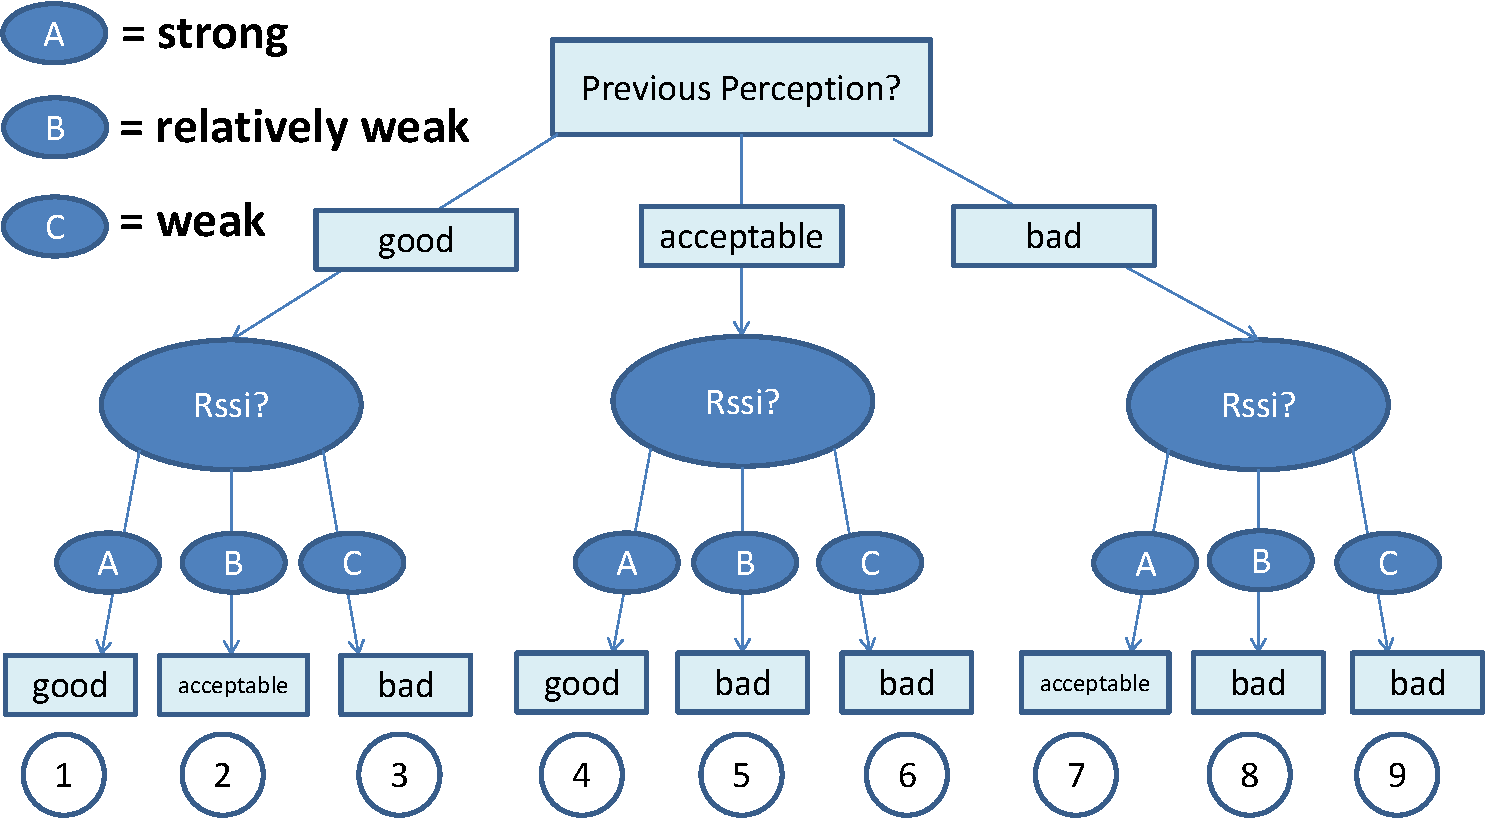
\includegraphics[scale=0.35]{updatePerception.pdf}
\caption{Decision tree for updating current perception of Wi-Fi}
\end{figure}

\section{Simulation Results}
In this section, we present our Monte Carlo simulation of the Rssi-based Wi-Fi download management algorithm and its detailed analysis.
\subsection{Simulation Methodology}
{\bf Halton Sequence}: Halton sequences are sequences used to generate points in space for numerical methods such as Monte Carlo simulations.
Although these sequences are deterministic they are of low discrepancy and appear to be random [11].
In our simulation, to simulate all possible starting point that a smartphone user could take, 
a 2-dimensional Halton sequence with base \{2, 3\} is generated. 
When the user get out of the signal range of the Wi-Fi AP, we consider one walk is terminated and take the next value of the Halton sequence 
as his new starting point. This process is characterized as:
\[ \vec{P}_{k_{t=0}} = R\textrm{H}_{k}(2, 3) \eqno(1) \]
where $R$ refers to the rayon of the signal range of the Wi-Fi AP. A starting point out of the range of the Wi-Fi is discarded and the user takes
the $k+1^{th}$ walk.
\\
\indent
{\bf Directional Random Walk}: To simulate the process of walk of a smartphone user, we introduce the directional random walk defined as:
$$ s_{k_{t}} \sim \textrm{U}(s_{min}, s_{max}) \eqno(2) $$
$$ \theta_{k_{t}} \sim \textrm{N}(\theta_{k_{t-1}}, \sigma^2) \eqno(3) $$
where $s_{k_{t}}$ and $\theta_{k_{t}}$ are respectively the speed and the heading of the smartphone user at instant $t$, drawn respectively 
from an uniform distribution and a Gaussian distribution. $\theta_{k_{t=0}}$ is set to be 0 as the signal range of the AP is a circle and 
therefore symmetric. (...) 
Thus the position of phone at the next instant can be given as:
\[ \vec{P}_{k_{t+1}} = \vec{P}_{k_{t}} + s_{k_{t}}{\cos\theta_{k_{t}} \choose \sin\theta_{k_{t}}} \eqno(4) \]
\\
\indent 
{\bf Stationary-Moving State Transition}: Considering that a smartphone user may use his phone not only in the move, but also when he 
is stationary, we introduce a Markov chain to characterize this stationary-moving transition, with two state spaces \textit{moving} and \textit{stationary} 
and the transition matrix:
%\[ \begin{pmatix}
%       p_{move} 	& 1-p_{move} \\
%       p_{stationary} 	& 1-p_{stationary}
%      \end{pmatix} \]
$$ 
A= \left(\begin{array}{lcr} p_{m} & 1-p_{m} \\
         1-p_{s} & p_{s} 	
      \end{array} \right) \eqno(5)
$$
where $p_{m}$ refers to the probability of the user continuing moving the next instant if he is on the move the current instant, and 
$p_{s}$ refers to the probability of the user staying stationary the next instant if he is stationary the current instant. 
Representing the \textit{moving} state as 1 and the \textit{stationary} state as 0, noted by $\delta \in$ \{0, 1\}, equation (4) can then be changed to:
\[ \vec{P}_{k_{t+1}} = \vec{P}_{k_{t}} + \delta_{k_{t+1}}s_{k_{t}}{\cos\theta_{k_{t}} \choose \sin\theta_{k_{t}}} \eqno(6) \]
\\
\indent
{\bf Rssi Variation Model}:
We adopt the logarithmic wireless path model to calculate the real Rssi of Wi-Fi from the distance between the AP and the smartphone:
$$ Rssi(d) = Rssi(d0) + 10\eta\log(d/d0) + \xi \eqno(7)$$
where d0 is the reference distance, typically 1 meter, $\eta$ is the path attenuation factor and $\xi$ the shadowing factor.
However, as each measurement of Rssi could introduce inaccuracy, we define Equation (8)-(10) to describe the variations of Rssi in measurements.
$$ d_{k_{t}} \sim \textrm{N}(0, \phi^2) \eqno(8) $$
$$ \Delta_{k_{t}} \equiv \lfloor\|d_{k_{t}}\|\rfloor \pmod{M}  \eqno(9) $$
$$ Rssi_{measured\_k_{t}}(d) = Rssi_{k_{t}}(d) + \textrm{sign}(d_{k_{t}})\Delta_{k_{t}} \eqno(10)$$
where $M$ refers to the maximum variation of measured Rssi from the real Rssi. 
For example, if the real Rssi is -20dBm and measured Rssi is \{-19dBm, -20dBm, -21dBm\}, 
then the $M$ is 1. 
Our experiments show that $M$ is 
5 if $Rssi(d)\in$ (-70dBm, -60dBm], 
6 if $Rssi(d)\in$ (-80dBm, -70dBm], 
7 if $Rssi(d)$ is lower than -80dBm.
So $M$ is given as:
$$M=\lfloor\|\frac{Rssi_{k_{t}}(d)}{10}\|\rfloor-1 \eqno(11)$$
\\
\indent
{\bf Monte-Carlo Simulation}: We simulate a person carrying 4 phones with him and performs 1,000,000 directional random walks in a plan with an AP in the center. 
Phone1 runs our algorithm for the download management.  
Phone2 starts the download if Rssi is measured to be strong and stops the download if Rssi is measured to be weak or relatively weak. 
Phone3 starts the download if Rssi is measured to be strong or relatively weak and stops the download if Rssi is measured to be weak.
Phone4 has no download strategy and keeps downloading regardless of Rssi. 
The 4 phones are all powered with 
a infinite-capacity battery, but their power consumptions are recorded. They are all the four charged with the task of downloading a file of infinite size. 
% \\
% \indent 
% Other specifications of the four phones are given in Table 2. Terms with * indicates that they are measured by Monsoon Power Monitor. 
\\
\indent
We incorporate our measurement results in our simulations, including the relationship between energy consumption and Rssi, the relationship between
throughput and Rssi, the tail energy and the variation of Rssi.
\\
\indent
Two simulations are carried out. In the first simulation, 
the person walks always and thus $p_{m}$ = 1, $p_{s}$ = 0. 
In the second simulation, the person walks and stops, with $p_{m}$ = 0.8, $p_{s}$ = 0.9. 

\subsection{Simulation Results}
{\bf First Simulation}: 
Our first simulation shows that in the constantly moving scenario, Phone1 will have 89.1\% of its download time spent in areas where the Wi-Fi signal is 
strong, 10.1\% in areas where the Wi-Fi signal is relatively weak, and 0\% in areas where the Wi-Fi signal is weak. The rate of being in 
strong Wi-Fi area and not downloading is 0.13\%.
\\
\indent
The size of file downloaded and the energy consumed by the 4 phones are shown in Figure 9 and Figure 10. We define the energy efficiency as 
the fraction of the size of file downloaded and the energy consumed, given in Equation (12). The energy efficiency of the 4 phones in the constantly moving scenario
is illustrated in Figure 11. 
$$ 
EnergyEfficiency = \frac{SizeOfFileDownloaded}{EnergyConsumed}	
\eqno(12)
$$
\begin{figure}
\centering
% \captionsetup{justification=centering}
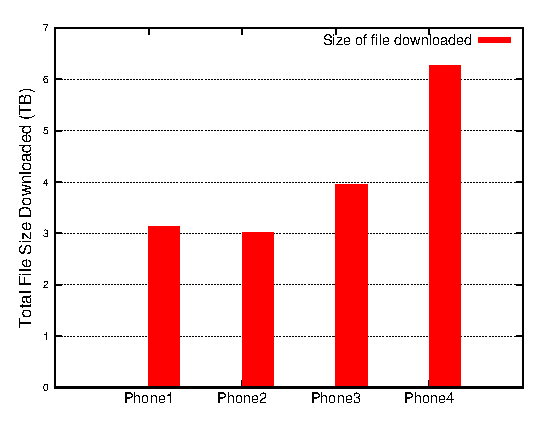
\includegraphics[scale=0.85]{result_directional_downloadsize.eps}
\caption{Size of file downloaded in Simulation1}
\end{figure}
\begin{figure}
\centering
% \captionsetup{justification=centering}
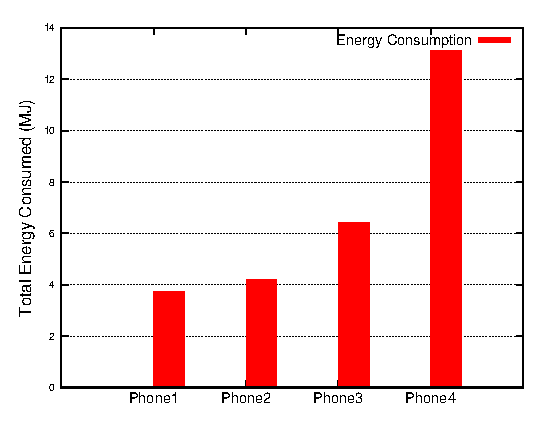
\includegraphics[scale=0.85]{result_directional_energy.eps}
\caption{Energy consumed for download in Simulation1}
\end{figure}
\begin{figure}
\centering
% \captionsetup{justification=centering}
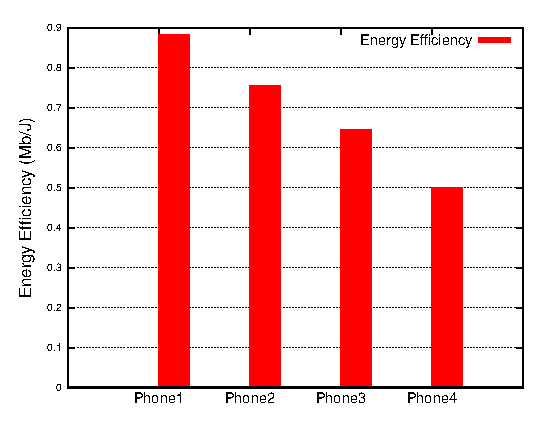
\includegraphics[scale=0.85]{result_directional_efficiency.eps}
\caption{Energy efficiency of the 4 phones in Simulation1}
\end{figure}
{\bf Second Simulation}: 
Our second simulation shows that in the stationary-moving Markov chain scenario, Phone1 will have 96.7\% of its download time spent in areas where the Wi-Fi signal is 
strong, 3.3\% in areas where the Wi-Fi signal is relatively weak, and 0\% in areas where the Wi-Fi signal is weak. The rate of being in 
strong Wi-Fi area and not downloading is 0.06\%. The size of file downloaded, 
the energy consumed, and the energy efficiency of the 4 phones are respectively shown in Figure 12, Figure 13 and Figure 14.
\begin{figure}
\centering
% \captionsetup{justification=centering}
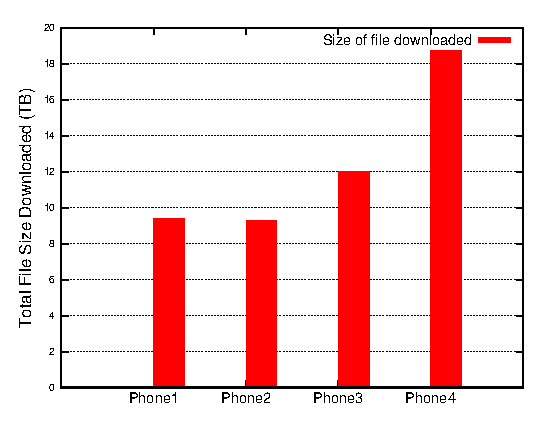
\includegraphics[scale=0.85]{result_markov_downloadsize.eps}
\caption{Size of file downloaded in Simulation2}
\end{figure}
\begin{figure}
\centering
% \captionsetup{justification=centering}
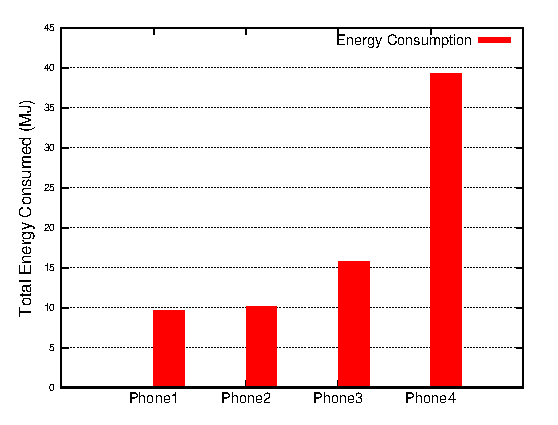
\includegraphics[scale=0.85]{result_markov_energy.eps}
\caption{Energy consumed for download in Simulation2}
\end{figure}
\begin{figure}
\centering
% \captionsetup{justification=centering}
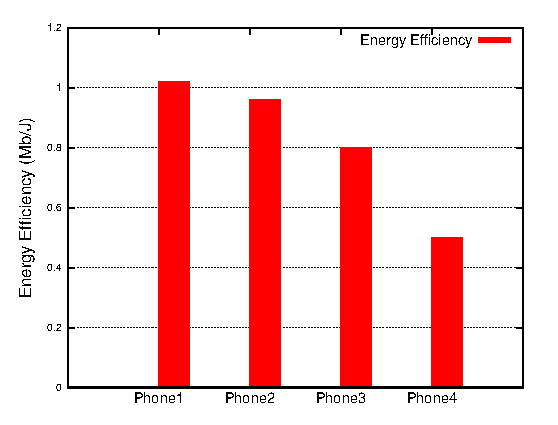
\includegraphics[scale=0.85]{result_markov_efficiency.eps}
\caption{Energy efficiency of the 4 phones in Simulation2}
\end{figure}
\subsection{Analysis of Simulation Results}
The performances of Phone2, Phone3 and Phone4 descrease, showing that even simple download controls according to Rssi can be effective.
We further analysis why Phone1 outperforms Phone2.
\\
\indent
Figure 14 and Figure 15 illustrate the number of download sessions and the average download session lengths of Phone1 and Phone2. We see that in Simulation1, 
Phone2 has 13.5\% more sessions than Phone1. This rate increases to 18.8\% in Simulation2. More session number
means more frequent transition between starting and stopping downloads, and wasting energy consumption in 
interrupting and reestablishing TCP connections as well as tail energy. 
At the same time, Phone1 also has 14.7\% longer average download session length than Phone2 in Simulation1 and 21.4\% in Simulation2. 
All these contribute to the better performance of Phone1 in preference to Phone2.
We conclude that our algorithm is effective in energy saving and succeed in fulfilling requirements of a good Rssi-based algorithm.
\begin{figure}
\centering
% \captionsetup{justification=centering}
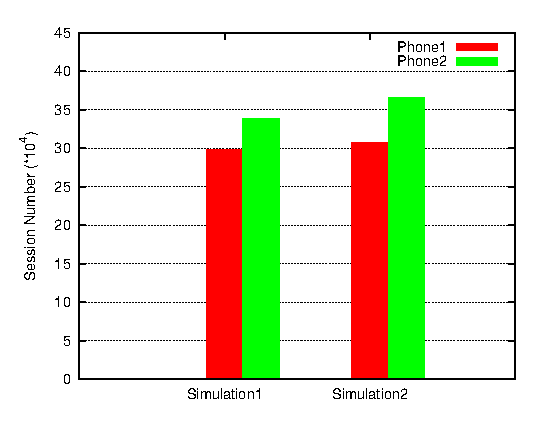
\includegraphics[scale=0.85]{comparison_session_number.eps}
\caption{Comparison of Phone1 and Phone2 in terms of download session number}
\end{figure}
\begin{figure}
\centering
% \captionsetup{justification=centering}
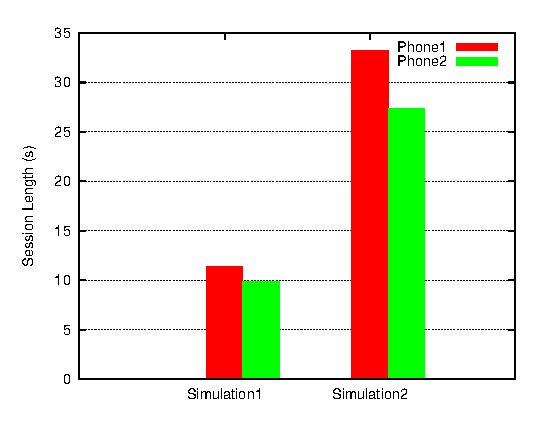
\includegraphics[scale=0.85]{comparison_session_length.eps}
\caption{Comparison of Phone1 and Phone2 in terms of average download session length}
\end{figure}
\section{Conclusion} 
In this paper, we first investigate the relationship between Rssi and energy consumption of smartphones
and then propose a novel Rssi-based Wi-Fi download management algorithm for energy savings.
Our algorithm, as simple as it is, incorporates some major characteristics of Wi-Fi signal.
Through Monte-Carlo simulations, we prove the effectiveness of our algorithm
and conclude that it leverages some main challenges such as varying nature of Rssi and
tail energy when stopping downloading. 
\section*{Acknowledgment}

This work is supported by the National Nature Science Foundation of China, NSFC (Grant No. 61170293) 
and the International Science \& Technology Cooperation Program of China, 
Ministry of Science and Technology of China (Grant No. 2014DFG12370).

\ifCLASSOPTIONcaptionsoff
  \newpage
\fi
\begin{thebibliography}{0}
\bibitem{biblio1}
Frank Vanheel et al., \emph{Automated linear regression tools improve RSSI WSN localization in multipath indoor environment}, 
\hskip 1em plus
  0.5em minus 0.4em\relax Journal on Wireless Communications and Networking, 2011

\bibitem{biblio1}
Noah Pritt, \emph{Indoor Positioning with Maximum Likelihood Classification of Wi-Fi Signals}, 
\hskip 1em plus
  0.5em minus 0.4em\relax SENSORS 2013 IEEE, November 2013, p1-p4

\bibitem{biblio1}
Doug Rosener, \emph{Decreasing Rssi Setting Time in Low-power Mode Systems}, 
\hskip 1em plus
  0.5em minus 0.4em\relax US Patent, Pub.No: US 2013/0029607 A1, Pub.Date: Jan 31, 2013  
  
\bibitem{biblio1}
Jenq-Shiou Leu, Nguyen Hai Tung, and Chun-Yao Liu, \emph{Non-Parametric RSS Prediction Based Energy Saving Scheme for Moving Smartphones}, 
\hskip 1em plus
  0.5em minus 0.4em\relax IEEE Transactions on Computers, July 2014, p1793-p1801
  
\bibitem{biblio1}
E. Tan, L. Guo, S. Chen, and X. Zhang, \emph{Psm-throttling: Minimizing energy consumption for bulk data communications in WLANs}, 
\hskip 1em plus
  0.5em minus 0.4em\relax IEEE International Conference on Network Protocols, October 2007, p123–p132

\bibitem{biblio1}
Fahad R. Dogar et al., \emph{Catnap: Exploiting High Bandwidth Wireless Interfaces to Save Energy for Mobile Devices}, 
\hskip 1em plus
  0.5em minus 0.4em\relax ACM MobiSys’10, June 15–18, 2010

\bibitem{biblio1}
Young-Seol Lee  and Sung-Bae Cho, \emph{An Efficient Energy Management System for Android Phone Using Bayesian Networks}, 
\hskip 1em plus
  0.5em minus 0.4em\relax IEEE International Conference on Distributed Computing Systems Workshops, 2012, p102-p107    

\bibitem{biblio1}
Jian Li et al., \emph{Application-Centric Wi-Fi Energy Management on Smart Phone}, 
\hskip 1em plus
  0.5em minus 0.4em\relax  Network Operations and Management Symposium (APNOMS), 2012 14th Asia-Pacific   

\bibitem{biblio1}
Monsoon Power Monitor, \emph{www.msoon.com/LabEquipment/PowerMonitor} 
\hskip 1em plus
  0.5em minus 0.4em\relax 
  
\bibitem{biblio1}
Di Zhang et al., \emph{Leveraging the Tail Time for Saving Energy in Cellular Networks},
\hskip 1em plus
  0.5em minus 0.4em\relax IEEE Transactions on Mobile Computing, July 2014, p1536-p1549
  
\bibitem{biblio1}
Halton Sequence, \emph{en.wikipedia.org/wiki/Halton\_sequence} 
\hskip 1em plus
  0.5em minus 0.4em\relax  
  
\end{thebibliography}

% [4] SiFi: Exploiting VoIP Silence for WiFi Energy Savings in Smart Phones

% [5] Anatomy of WiFi Access Traffic of Smartphones and Implications for Energy Saving Techniques

\end{document}


